\documentclass[journal,12pt,twocolumn]{IEEEtran}
\usepackage{setspace}
\usepackage{gensymb}
\usepackage{xcolor}
\usepackage{caption}
\singlespacing
\usepackage{siunitx}
\usepackage[cmex10]{amsmath}
\usepackage{mathtools}
\usepackage{hyperref}
\usepackage{amsthm}
\usepackage{mathrsfs}
\usepackage{txfonts}
\usepackage{stfloats}
\usepackage{cite}
\usepackage{cases}
\usepackage{subfig}
\usepackage{longtable}
\usepackage{multirow}
\usepackage{enumitem}
\usepackage{bm}
\usepackage{mathtools}
\usepackage{listings}
\usepackage{tikz}
\usetikzlibrary{matrix}
\renewcommand{\vec}[1]{\boldsymbol{\mathbf{#1}}}
\DeclareMathOperator*{\Res}{Res}
\renewcommand\thesection{\arabic{section}}
\renewcommand\thesubsection{\thesection.\arabic{subsection}}
\renewcommand\thesubsubsection{\thesubsection.\arabic{subsubsection}}

\renewcommand\thesectiondis{\arabic{section}}
\renewcommand\thesubsectiondis{\thesectiondis.\arabic{subsection}}
\renewcommand\thesubsubsectiondis{\thesubsectiondis.\arabic{subsubsection}}
\hyphenation{op-tical net-works semi-conduc-tor}

\lstset{
language=Python,
frame=single, 
breaklines=true,
columns=fullflexible
}
\begin{document}
\theoremstyle{definition}
\newtheorem{theorem}{Theorem}[section]
\newtheorem{problem}{Problem}
\newtheorem{proposition}{Proposition}[section]
\newtheorem{lemma}{Lemma}
\newtheorem{corollary}[theorem]{Corollary}
\newtheorem{example}{Example}[section]
\newtheorem{definition}{Definition}[section]
\newcommand{\BEQA}{\begin{eqnarray}}
\newcommand{\EEQA}{\end{eqnarray}}
\newcommand{\define}{\stackrel{\triangle}{=}}
\newcommand{\myvec}[1]{\ensuremath{\begin{pmatrix}#1\end{pmatrix}}}
\newcommand{\mydet}[1]{\ensuremath{\begin{vmatrix}#1\end{vmatrix}}}
\bibliographystyle{IEEEtran}
\providecommand{\nCr}[2]{\,^{#1}C_{#2}} % nCr
\providecommand{\nPr}[2]{\,^{#1}P_{#2}} % nPr
\providecommand{\mbf}{\mathbf}
\providecommand{\pr}[1]{\ensuremath{\Pr\left(#1\right)}}
\providecommand{\qfunc}[1]{\ensuremath{Q\left(#1\right)}}
\providecommand{\sbrak}[1]{\ensuremath{{}\left[#1\right]}}
\providecommand{\lsbrak}[1]{\ensuremath{{}\left[#1\right.}}
\providecommand{\rsbrak}[1]{\ensuremath{{}\left.#1\right]}}
\providecommand{\brak}[1]{\ensuremath{\left(#1\right)}}
\providecommand{\lbrak}[1]{\ensuremath{\left(#1\right.}}
\providecommand{\rbrak}[1]{\ensuremath{\left.#1\right)}}
\providecommand{\cbrak}[1]{\ensuremath{\left\{#1\right\}}}
\providecommand{\lcbrak}[1]{\ensuremath{\left\{#1\right.}}
\providecommand{\rcbrak}[1]{\ensuremath{\left.#1\right\}}}
\theoremstyle{remark}
\newtheorem{rem}{Remark}
\newcommand{\sgn}{\mathop{\mathrm{sgn}}}
\newcommand{\rect}{\mathop{\mathrm{rect}}}
\newcommand{\sinc}{\mathop{\mathrm{sinc}}}
\providecommand{\abs}[1]{\left\vert#1\right\vert}
\providecommand{\res}[1]{\Res\displaylimits_{#1}} 
\providecommand{\norm}[1]{\left\Vert#1\right\Vert}
\providecommand{\mtx}[1]{\mathbf{#1}}
\providecommand{\mean}[1]{E\left[ #1 \right]}
\providecommand{\fourier}{\overset{\mathcal{F}}{ \rightleftharpoons}}
\providecommand{\ztrans}{\overset{\mathcal{Z}}{ \rightleftharpoons}}
\providecommand{\system}[1]{\overset{\mathcal{#1}}{ \longleftrightarrow}}
\newcommand{\solution}{\noindent \textbf{Solution: }}
\providecommand{\dec}[2]{\ensuremath{\overset{#1}{\underset{#2}{\gtrless}}}}
\let\StandardTheFigure\thefigure
\def\putbox#1#2#3{\makebox[0in][l]{\makebox[#1][l]{}\raisebox{\baselineskip}[0in][0in]{\raisebox{#2}[0in][0in]{#3}}}}
     \def\rightbox#1{\makebox[0in][r]{#1}}
     \def\centbox#1{\makebox[0in]{#1}}
     \def\topbox#1{\raisebox{-\baselineskip}[0in][0in]{#1}}
     \def\midbox#1{\raisebox{-0.5\baselineskip}[0in][0in]{#1}}

\vspace{3cm}
\title{Linear Programming Assignment}
\author{Gautam Singh}
\maketitle
\bigskip

\begin{abstract}
    This document contains the solution to Question 10 of 
    Exercise 1 in Chapter 12 of the class 12 NCERT textbook.
\end{abstract}

\begin{enumerate}
    \item Maximise 
    \begin{align}
        Z = x + y
        \label{eq:func}
    \end{align}
    subject to 
    \begin{align}
        x - y &\le -1 \label{eq:constr1} \\
        -x + y &\le 0 \label{eq:constr2} \\
        x, y &\ge 0
    \end{align}

    \solution We use the simplex method. Introducing slack variables,
    we rewrite \eqref{eq:func}, \eqref{eq:constr1} and \eqref{eq:constr2}.
    \begin{align}
        x - y + s_1 &= -1 \\
        -x + y + s_2 &= 0 \\
        -x - y + Z &= 0 \\
        x, y, s_1, s_2, Z &\ge 0
    \end{align}

    The augmented matrix becomes
    \begin{align}
        \vec{S} = 
        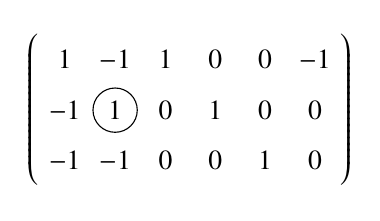
\begin{tikzpicture}[baseline]
        \matrix[
            matrix of math nodes, 
            minimum size=16pt,
            row sep=2pt,
            column sep=2pt,
            left delimiter=(,
            right delimiter=), 
            inner xsep=0pt,
            ampersand replacement = \&
            ]{
            1 \& -1 \& 1 \& 0 \& 0 \& -1 \\
            -1 \& |[draw, circle]|1 \& 0 \& 1 \& 0 \& 0 \\
            -1 \& -1 \& 0 \& 0 \& 1 \& 0 \\
            };
        \end{tikzpicture}
        \label{eq:simplex-aug}
    \end{align}
    Here, choosing the pivot column of $\vec{S}$ to be the second column, 
    the ratios by row numbers are
    \begin{align}
        r_1 &= \frac{-1}{1} = -1 \label{eq:r1} \\
        r_2 &= \frac{0}{1} = 0 \label{eq:r2} \\
        r_3 &= \frac{0}{-1} = 0 \label{eq:r3}
    \end{align}
    From \eqref{eq:r1} to \eqref{eq:r3}, we see that row 2 is suitable to be
    assigned a pivot row. Hence, the pivot element is circled in 
    \eqref{eq:simplex-aug}. By row reduction,
    \begin{align}
        \vec{S} &\xleftrightarrow{R_1 \leftarrow R_1 + R_2} \myvec{0&0&1&1&0&-1\\-1&1&0&1&0&0\\-1&-1&0&0&1&0} \\
                &\xleftrightarrow{R_3 \leftarrow R_3 + R_2} \myvec{0&0&1&1&0&-1\\-1&1&0&1&0&0\\-2&0&0&0&1&0}
                \label{eq:S-red}
    \end{align}
    Again, the pivot column in \eqref{eq:S-red} is the first column. However, 
    the first column has all negative elements, and therefore, there is no solution 
    to the optimization problem. This is justified by Fig. \ref{fig:lp}, plotted
    using the Python code \texttt{codes/lp.py}.
    \begin{figure}[!ht]
        \centering
        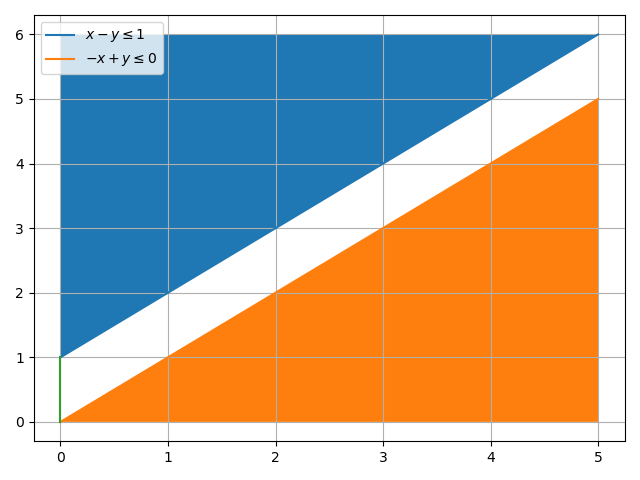
\includegraphics[width=\columnwidth]{figs/lp.png}
        \caption{The given optimization problem has no solution.}
        \label{fig:lp}
    \end{figure}
    This is also verified using \textit{cvxpy} in the Python code \texttt{codes/lp\_cvx.py}.
\end{enumerate}
\end{document}
